\PassOptionsToPackage{subsection=false}{beamerouterthememiniframes}
\documentclass{beamer}
%\documentclass{article} \usepackage{beamerarticle}
\usepackage[utf8x]{inputenc}
\usepackage[mongolian]{babel}
\usepackage{ifthen,graphicx,color,amssymb,multirow,xfrac,subcaption,tikz,pgfplots,listings,fontawesome,multicol,url}

\usepackage{array}
\newcolumntype{L}[1]{>{\raggedright\let\newline\\\arraybackslash\hspace{0pt}}m{#1}}
\newcolumntype{C}[1]{>{\centering\let\newline\\\arraybackslash\hspace{0pt}}m{#1}}
\newcolumntype{R}[1]{>{\raggedleft\let\newline\\\arraybackslash\hspace{0pt}}m{#1}}

\mode<presentation>{
 \usetheme{Boadilla} \usecolortheme{beaver}
 \addtobeamertemplate{background canvas}{\transfade[duration=1]}{}
 %\setbeamercolor{footnote}{fg=red}
 \setbeamercolor{footnote mark}{fg=red}
 \usenavigationsymbolstemplate{}
 \setbeamertemplate{itemize items}[default]
 \setbeamertemplate{enumerate items}[default]
 \setbeamertemplate{title page}[default]
 \setbeamertemplate{blocks}[default]
}

\makeatletter
\expandafter\let\csname beamer@@tmpop@theorem begin@numbered\endcsname\relax
\defbeamertemplate{theorem begin}{numbered}
{%
  \begin{\inserttheoremblockenv}
    {%
      \inserttheoremname\hspace{-0.6em}
      %inserttheoremnumber
      \ifx\inserttheoremname\@empty\else\ \ifx\inserttheoremaddition\@empty\else\ \hspace{-0.35em}:\fi\hspace{-0.45em} \fi
      \ifx\inserttheoremaddition\@empty\else\ \inserttheoremaddition\fi% (\inserttheoremaddition)
    }%
}
\makeatother
\setbeamertemplate{theorems}[numbered]

\deftranslation[to=mongolian]{Definition}{Тодорхойлолт}
\deftranslation[to=mongolian]{Theorem}{Теорем}
\deftranslation[to=mongolian]{Lemma}{Лемм}
\deftranslation[to=mongolian]{Corollary}{Мөрдлөгөө}
\deftranslation[to=mongolian]{Example}{Жишээ}
\deftranslation[to=mongolian]{Problem}{Бодлого}

\lstset{
  language=R,
  basicstyle={\ttfamily},
%  backgroundcolor=\color{black!25},
  keywordstyle=\color{blue!85},
  commentstyle=\color{red!85},
  stringstyle=\color{black!75},
  breakatwhitespace=true,
  breaklines=true,
  frame=l,
  framesep=5pt,framerule=1pt,
  xleftmargin=7pt,xrightmargin=0pt,
  rulecolor=\color{blue!65},
  keepspaces=true,
  showstringspaces=false,
  columns=flexible,
  numbers=none,
  tabsize=3,
  otherkeywords={},
  deletendkeywords={},
  deletekeywords={}
}

\definecolor{darkred}{RGB}{114,0,0}

\newcommand{\copyrightyear}{2016}

\title[Симуляцийн аргууд]{Симуляцийн аргууд хичээлийн бие даалтын ажил}
\subtitle{IIE/RA Contest Problem 3: Sally Model's SM Pizza Shop}
\author{Г.Махгал}
\institute[]{МУИС -- ХШУИС -- Хэрэглээний Математикийн Тэнхим}
\logo{
\begin{tikzpicture}[scale=0.5,rotate=135]
 \draw [white,fill=darkred] (0,0) -- (0,1) -- (1,1) -- (1,0) -- (0,0);
 \draw [white,fill=white] (0.25,0) -- (0.25,0.8) -- (0.55,0.8) -- (0.55,1) -- (0.75,1) -- (0.75,0.6) -- (0.45,0.6) -- (0.45,0) -- (0.25,0);
\end{tikzpicture}
}
\date[Бие даалтын ажил]{\tiny \faCodeFork\ \the\year/\the\month/\the\day}

\begin{document}

\frame{\titlepage}

\frame
{\frametitle{}\framesubtitle{}
\begin{abstract}
\begin{itemize}
\item IIE/RA Contest Problem 3: Sally Model's SM Pizza Shop бодлогыг авч үзэх болно.
\item Бодлогыг програмчлалын R хэл\footnote{\url{https://en.wikipedia.org/wiki/R_(programming_language)}} дээр бодсон.
\item Хугацааны нэгжийг минутаар авсан.
\item Энэхүү слайд болон бодлогын өгүүлбэр, холбогдох өгөгдөл, R хэл дээрх код зэргийг
\\ {\color{blue}\url{https://github.com/galaamn/source-code-on-statistics/tree/master/Simulation/Example/Pizza\%20Shop}}
\\
хаягаар интернэтэд байрлуулсан.
\item Цаашид зуухны хэсгийн загварчлалыг сайжруулах шаардлагатай.
\end{itemize}
\end{abstract}
}

\frame
{\frametitle{Бодлого}\framesubtitle{Пицца хийж борлуулдаг дэлгүүр}
\begin{itemize}
\item Өгөгдөхүүн
\begin{itemize}
\item Ихдээ 3 хүн ажиллах боломжтой пицца бэлдэх ширээ
\item Гурван төрлийн сонголттой\footnote{оруулах хэсгийн багтаамжаараа ялгагдана} нэг зуух
\item Хүргэлтийн ажилчид
\end{itemize}
\item Бусад
\begin{itemize}
\item Захиалгын эрчим
\item Захиалга дахь пиццаны тоо болон хэмжээ тус бүрийн тархалтууд\footnote{эдгээр хувьсагчид дээр хамаарлын талаар ямар нэг зүйл дурдагдаагүй байна}
\item Пицца бэлдэх ажлын шат дамжлагууд, тэдгээрийн үргэлжлэх хугацааны тархалт
\item Пиццаг хэрчиж савлахад зарцуулагдах хугацааны тархалт
\item Хүргэлтийн хугацааны тархалт
\end{itemize}
\item Олох зүйл
\begin{itemize}
\item Пицца бэлдэх ширээнд ажиллуулах хүний тоо
\item Зуухны төрөл
\item Пицца хүргэлтэнд ажиллах хүний тоо
\end{itemize}
\end{itemize}
}

\begin{frame}[fragile]
\frametitle{Санамсаргүй хувьсагчийн загварчлал}\framesubtitle{Гурвалжин тархалт\footnote{\url{https://en.wikipedia.org/wiki/Triangular_distribution}}}
\begin{figure}
\begin{tikzpicture}
\draw [->] (0,0) -- (4,0);
\draw [->] (0,0) -- (0,2);
\draw [blue] (0.5,0) node [below,black] {$a$} -- (2.5,1.75) -- (3.5,0) node [below,black] {$b$};
\draw [dashed] (0,1.75) node [left] {$\frac{2}{b-a}$} -- (2.5,1.75) -- (2.5,0) node [below] {$c$};
\node at (4,1) [right] {$F(x)=\left\{
\begin{array}{ll}
0 & x\leq a \\
\frac{(x-a)^2}{(b-a)(c-a)} & a<x\leq c \\
1-\frac{(b-x)^2}{(b-a)(b-c)} & c<x<b \\
1 & b\leq x
\end{array}
\right.$};
\end{tikzpicture}
\end{figure}
\vskip-2mm
Урвуу хувиргалтын аргаар
\begin{lstlisting}[keywords={function,ifelse,runif,sqrt}]
rtriangular = function (n, a, c, b) {
  ifelse(
    (u = runif(n)) < (c-a)/(b-a),
    a + sqrt((b-a)*(c-a)*u),
    b - sqrt((b-a)*(b-c)*(1-u))
  )
}
\end{lstlisting}
\end{frame}

\begin{frame}[fragile]
\frametitle{Санамсаргүй хувьсагчийн загварчлал}\framesubtitle{Бусад}
\begin{itemize}
\item Жигд тархалт буюу санамсаргүй тоо \\ R програмын \texttt{stats} багц дахь \lstinline|runif()| функц
\item Тархалтуудын холимог\footnote{composition method} \\ Хоёр ширхэг гурвалжин тархалтын холимог\footnote{хэрчиж савлах хэсэгт}
\item Илтгэгч тархалт \\ R програмын \texttt{stats} багц дахь \lstinline|rexp()| функц\footnote{захиалга хоорондын хугацааг загварчлахад ашиглагдана}
\end{itemize}
\end{frame}

\begin{frame}[fragile]
\frametitle{Загварчлалын үе шатууд}\framesubtitle{}
\footnotesize
\begin{enumerate}
\item Захиалга орж ирэх хугацааны эгшинг загварчлах \\ {\scriptsize захиалгын эрчимд тохируулан захиалга хоорондын хугацааг тодорхойлно}
\item Захиалгын зарим мэдээлэл \\ {\scriptsize пиццаны тоо ба хэмжээ, захиалгын төрөл (delivery эсвэл carry-out), хүргэлтийн хугацаа}
\item Пиццаны зарим мэдээлэл \\ {\scriptsize пицца нэг бүрийн хэмжээ болон хийхэд зарцуулагдах хугацаа (3 үе шат нэг бүрчлэн)}
\item Пиццаг бэлдэх ажлыг загварчлах \\ {\scriptsize пицца хийх ширээнд ажиллах хүний тооноос (1-ээс 3 хүртэл) хамаарна}
\item Зуухны хэсгийг загварчлах \\ {\scriptsize пицца нэг бүрийн зуухны оруулах хэсэгт нэвтрэх эгшин болон зуухны гаргах хэсэгт шилжих эгшин}
\item Хэрчиж савлах, захиалгыг гаргах хэсгийг загварчлах \\ {\scriptsize IIE\_SM\_3.dat файл дахь өгөгдлийг шинжилж улмаар зохих тархалтын тусламжтайгаар энэ хэсэгт зарцуулагдах хугацааг тодорхойлно}
\item Хүргэлтийн хэсгийг загварчлах \\ {\scriptsize захиалгыг хүргэхэд зарцуулагдах хугацааг тодорхойлно, хүргэлтийн ажилчдын тоо хувьсах боломжтой байх шаардлагатай}
\item Захиалгыг гүйцэтгэхэд зарцуулсан нийт хугацааг олох
\end{enumerate}
\end{frame}

\begin{frame}[fragile]
\frametitle{Үр дүн}\framesubtitle{Захиалгын тооны зарим статистик үзүүлэлтүүд}
\begin{itemize}
\item Дундаж
\begin{lstlisting}[morekeywords={in}]
the.number.of.demands = c()
for (i in 1:1000) {
  the.number.of.demands = c(the.number.of.demands, length(simulate.demands()))
}
mean(the.number.of.demands)
\end{lstlisting}
\begin{lstlisting}
120.303
\end{lstlisting}
энд \lstinline|simulate.demands()| -- захиалгыг загварчлах функц
\item Стандарт хазайлт
\begin{lstlisting}
sd(the.number.of.demands)
\end{lstlisting}
\begin{lstlisting}
10.86505
\end{lstlisting}
\end{itemize}
\end{frame}

\begin{frame}[fragile]
\frametitle{Үр дүн}\framesubtitle{Захиалгыг бүрэн гүйцэтгэх хугацааны зарим үзүүлэлт, параметрийн зарим утганд}
Ашиглагдах код
\begin{lstlisting}[keywords={c,for,in,switch}]
elapsed.time = demand.type = c()
for (i in 1:1000) {
  demands = simulate.demands()
  demands = simulate.count.and.size(demands)
  pizzas = simulate.pizza.making(demands)
  pizzas = switch(the.number.of.person.at.make.table, pizza.making.one.person(), pizza.making.two.person(), pizza.making.three.person())
  oven(); cut.and.box(); delivery()
  demands$elapsed.time = demands[["delivery.time"]] - demands[["time"]]
  elapsed.time = c(elapsed.time, demands[["elapsed.time"]])
  demand.type = c(demand.type, demands[["type"]])
}
\end{lstlisting}
\end{frame}

\begin{frame}[fragile]
\frametitle{Үр дүн}\framesubtitle{Захиалгыг бүрэн гүйцэтгэх хугацааны зарим үзүүлэлт, параметрийн зарим утганд}
Ашиглагдах код
\begin{lstlisting}[keywords={tapply,mean,range}]
tapply(elapsed.time, demand.type, mean)
tapply(elapsed.time, demand.type, range)
\end{lstlisting}
\vskip-2mm
\begin{table}
\begin{tabular}{ccc|rrr|rrr}
\multirow{2}{*}{\faMale\footnote{Ширээн дэх ажилчдын тоо}} & \multirow{2}{*}{\faFire\footnote{Зуухны төрөл}} & \multirow{2}{*}{\faMotorcycle\footnote{Хүргэгчдийн тоо}} & \multicolumn{3}{c|}{delivery} & \multicolumn{3}{c}{carry-out} \\
& & & mean & min & max & mean & min & max \\
\hline
1 & 3 & 7 & 115.02 & 16.31 & 299.16 & 108.42 & 12.59 & 289.28 \\
2 & 3 & 7 & 39.57 & 15.97 & 112.57 & 32.06 & 12.35 & 101.92 \\
3 & 1 & 5 & 46.95 & 15.97 & 149.52 & 23.36 & 12.40 & 74.67 \\
3 & 1 & 6 & 37.09 & 16.16 & 113.10 & 23.56 & 12.38 & 75.37 \\
3 & 1 & 7 & 32.82 & 15.91 & 86.42 & 23.43 & 12.37 & 71.54 \\
3 & 3 & 7 & 31.12 & 16.37 & 79.40 & 21.47 & 12.40 & 69.97 \\
3 & 3 & 8 & 28.96 & 16.04 & 67.95 & 21.24 & 12.38 & 63.03 \\
\end{tabular}
\end{table}
\end{frame}

\begin{frame}[fragile]
\frametitle{Үр дүн}\framesubtitle{Захиалгыг бүрэн гүйцэтгэх хугацааны зарим үзүүлэлт, параметрийн 3, 1, 7 утганд}
Ашиглагдах код
\begin{lstlisting}[keywords={tapply,boxplot}]
tapply(elapsed.time, demand.type, quantile, probs = 0.9)
boxplot(formula = elapsed.time ~ demand.type)
\end{lstlisting}
Үр дүн
\begin{lstlisting}[keywords={tapply,boxplot}]
47.17 # delivery
35.12 # carry-out
\end{lstlisting}
\vskip-8mm
\begin{figure}
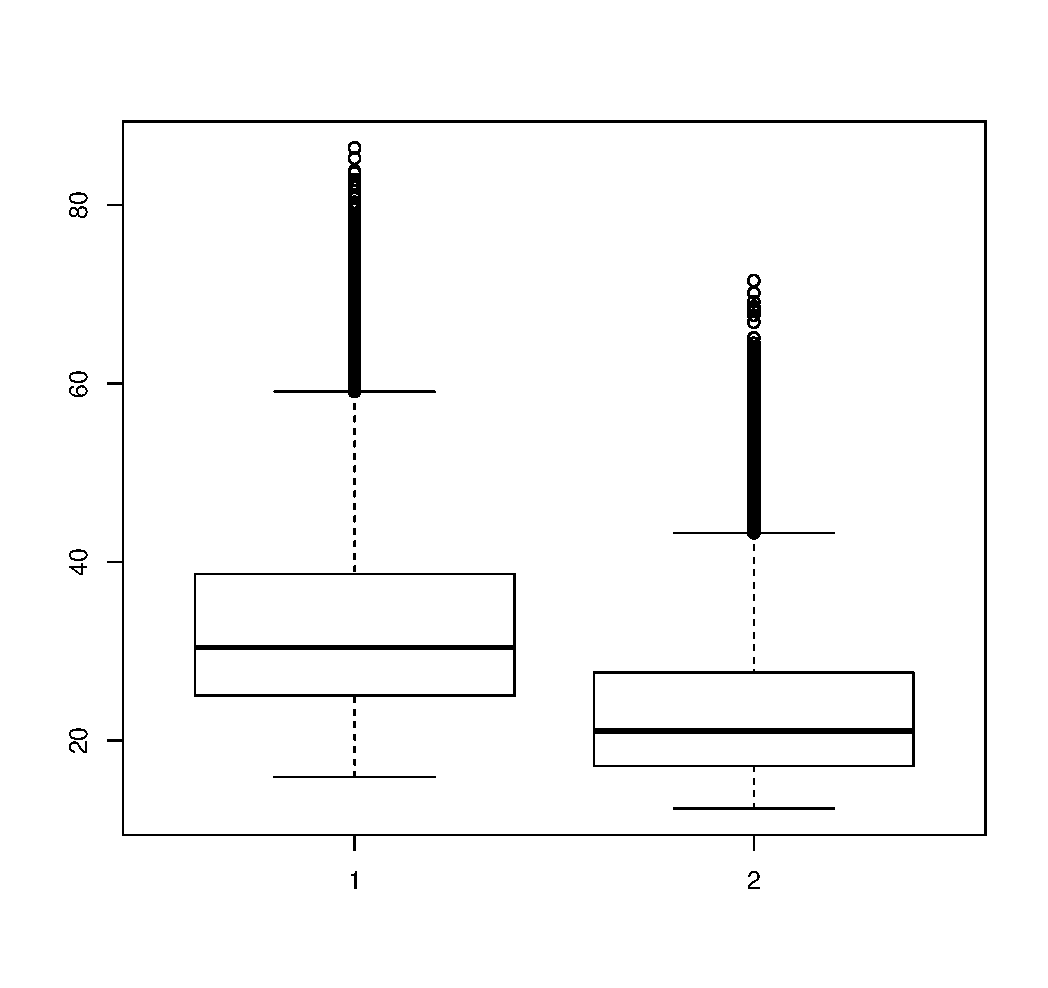
\includegraphics[width=0.425\textwidth]{boxplot}
\end{figure}
\end{frame}

\frame
{
\begin{center}
\scalebox{10}{\color{darkred}\faSmileO}
\end{center}
}
\end{document}